\documentclass[10pt,journal]{IEEEtran}
\usepackage[T1]{fontenc}
\usepackage[utf8]{inputenc}
\usepackage{amsmath,amssymb,graphicx,booktabs,tabularx,array}
\usepackage{cite,flushend}
\usepackage{placeins}
\renewcommand{\arraystretch}{1.08}
\usepackage{microtype}
\usepackage[hidelinks]{hyperref}
\hypersetup{pdftitle={Revocable Face Templates Under Multiple Exposures: Utility, Linkability, and Inversion},pdfauthor={Abhishek A. K.},pdfsubject={Research manuscript for author review},pdfkeywords={biometric template protection, face verification, revocation, template inversion}}
\graphicspath{{figures/}}
\newcommand{\norm}[1]{\left\lVert#1\right\rVert_2}
\newcommand{\unit}{\operatorname{unit}}
\newcommand{\ASR}{\operatorname{ASR}}
\newcommand{\FAR}{\operatorname{FAR}}
\newcommand{\TAR}{\operatorname{TAR}}
\newcommand{\tabnote}[1]{\par\vspace{3pt}\begin{minipage}{\linewidth}\footnotesize\raggedright #1\end{minipage}}
% Generated by editorial_metrics.py from included CSV evidence.
\newcommand{\MbfSmallTar}{37.76--43.50\%}
\newcommand{\MbfSmallAsr}{18.84--32.96\%}
\newcommand{\RnetSmallTar}{65.12--66.94\%}
\newcommand{\RnetSmallAsr}{38.28--53.09\%}
\newcommand{\MbfLargeTar}{81.95--82.52\%}
\newcommand{\MbfLargeAsr}{77.52--78.56\%}
\newcommand{\RnetLargeTar}{94.37--94.67\%}
\newcommand{\RnetLargeAsr}{92.03--92.30\%}
\newcommand{\LfwBaselineAsr}{64.53--80.96\%}

\newcommand{\fignote}[1]{\par\vspace{2pt}\begin{minipage}{\linewidth}\footnotesize\raggedright #1\end{minipage}}
% Compact float placement without stretching inter-figure white space.
\setcounter{topnumber}{4}
\setcounter{dbltopnumber}{4}
\setcounter{totalnumber}{6}
\renewcommand{\topfraction}{.90}
\renewcommand{\dbltopfraction}{.90}
\renewcommand{\textfraction}{.08}
\renewcommand{\floatpagefraction}{.75}
\renewcommand{\dblfloatpagefraction}{.75}
\setlength{\floatsep}{10pt plus 2pt minus 2pt}
\setlength{\dblfloatsep}{10pt plus 2pt minus 2pt}
\setlength{\textfloatsep}{12pt plus 2pt minus 2pt}
\setlength{\dbltextfloatsep}{12pt plus 2pt minus 2pt}
\makeatletter
\setlength{\@fptop}{0pt}
\setlength{\@fpsep}{12pt}
\setlength{\@fpbot}{0pt plus 1fil}
\setlength{\@dblfptop}{0pt}
\setlength{\@dblfpsep}{12pt}
\setlength{\@dblfpbot}{0pt plus 1fil}
\makeatother
\begin{document}
\title{Revocable Face Templates Under Multiple Exposures: Utility, Linkability, and Inversion}
\author{Abhishek A. K.\\[0.6ex]
{\normalfont\small Department of Computer Science and Engineering, Manipal Institute of Technology,\\
Manipal Academy of Higher Education, Manipal, India\\
Department of Computer Science and Engineering,\\
Indian Institute of Information Technology Dharwad, Dharwad, India}}
\maketitle
\begin{abstract}
Changing a compromised face template does not necessarily remove the information revealed by its earlier versions. We examine this problem through a joint evaluation of repeated-exposure reconstruction, recognition, and compact-reference storage. The experiments apply random orthogonal, subsampled randomized Hadamard, and PCA-guided projections to frozen MobileFaceNet and ResNet50 ArcFace embeddings. Packed 128-bit and 512-bit templates occupy 16 and 64 bytes, respectively, in place of a 2048-byte raw embedding. With ten historical exposures, calibrated cross-image fresh-key attack success in the original 128-bit LFW study reaches \LfwBaselineAsr{}. In the matched screened-CFP experiment, ResNet50 achieves protected true acceptance of \RnetSmallTar{} at 128 bits and \RnetLargeTar{} at 512 bits. Its corresponding ten-exposure attack success is \RnetSmallAsr{} and \RnetLargeAsr{}, compared with \MbfSmallAsr{} and \MbfLargeAsr{} for MobileFaceNet. Reconstruction uses historical operators but has no access to the fresh operator. Conditional identity-bootstrap intervals and paired contrasts quantify uncertainty within the fixed protocols. The findings separate successful invalidation of an old record from resistance to recovery of useful identity information. They also show why compact-template selection requires recognition and security evidence alongside payload savings. On-device latency, memory, energy, and camera-level attacks are not evaluated.
\end{abstract}
\begin{IEEEkeywords}
Biometric template protection, cancellable biometrics, face verification, revocation, template inversion, resource-constrained edge systems.
\end{IEEEkeywords}
\section{Introduction}\label{sec:introduction}
\IEEEPARstart{F}{ace} verification compares an image of a person with a reference associated with a claimed identity. After detection and alignment, an encoder maps the face to a feature vector on which the matching decision is based. Learned representations have substantially advanced recognition~\cite{deepface,facenet,arcface}, but their identity content also creates a security concern: a disclosed vector can reveal information beyond the comparison for which it was collected. Face reconstruction from embeddings has been demonstrated in prior work~\cite{mai2019reconstruction,vec2face,shahreza2024adapter}. Replacing an exposed reference is therefore more difficult than resetting a password, because the person's biometric characteristic persists.

Cancellable biometrics introduce a replaceable transformation between the biometric features and the stored reference~\cite{ratha2001enhancing,ratha2007cancelable}. Changing its key allows a system to issue a new template after compromise. Renewal, however, is only one protection requirement. The transformed representation must also retain useful recognition performance, limit associations across records, and resist recovery of identity-bearing information. An obsolete template may be rejected while still revealing information useful for a subsequent attack. We use the terminology of biometric protection standards to distinguish these properties, without asserting formal compliance~\cite{iso24745,iso30136}.

Storage constraints make binary references attractive for edge applications such as public kiosks and smart gadgets. MobileFaceNet supplies a compact baseline encoder~\cite{chen2018mobilefacenet}; its 512-dimensional float32 output requires 2048 bytes, whereas packed 128-bit and 512-bit templates require 16 and 64 bytes. This difference becomes relevant when a device retains many references. Whether the reduction is useful nevertheless depends on the recognition performance retained and the consequences of compromise. The payload also represents only part of the resource requirement: model weights, working memory, projection operators, keys, and metadata incur additional costs.

Successive renewals can leave an adversary with several observations of the same underlying feature vector. If historical transformation operators are also exposed, hiding the current operator does not remove those observations. One-bit recovery theory explains how signs retain directional information~\cite{plan2013,jacques2013}, and pre-image and record-multiplicity attacks provide established examples of this concern~\cite{wang2021csa,li2014multiplicity}. The question examined here is how historical exposure affects renewed verification when template length, recognition utility, and encoder choice are considered together.

The study evaluates random orthogonal (RO), subsampled randomized Hadamard (SRHT), and PCA-guided RO projections on LFW and CFP-FP~\cite{huang2007lfw,sengupta2016cfp}. It compares MobileFaceNet with a ResNet50 ArcFace checkpoint under matched inputs within each encoder experiment. Official benchmark recognition and custom attack protocols are reported separately. The screened CFP attack pool contains 5704 crops from 500 identities. LFW attack results use MobileFaceNet; the two-encoder attack comparison is limited to CFP.


Renewal changes the protected reference and its operator while leaving the encoder's identity information in place. A version gate can invalidate the old record at the system interface, yet an attacker may continue to use its measurements offline. Direct replay consequently tests only whether the old bits still match; it does not test whether those bits help construct a new submission. Our evaluation treats these as separate questions and assigns a distinct outcome measure to each.

The evaluation also distinguishes the information available to each adversary. A template-only attacker attempts to associate binary records without knowing their operators. An inversion attacker receives the compromised operators and can exploit their signed constraints on the feature vector. Weak discrimination in the first setting cannot establish resistance in the second. Keeping the fresh operator unavailable during reconstruction tests whether the information retained from earlier transformations is sufficient to support acceptance after renewal.

Encoder choice complicates the interpretation of attack acceptance. A checkpoint that better matches genuine images may also match a reconstructed embedding more readily, even when reconstruction cosine changes little. Acceptance thus depends on both the recovered information and the recognition pipeline through which it is assessed. We align images, key schedules, and evaluation rules across the two encoders, while fitting preprocessing and thresholds separately on the permitted data. This compares complete frozen pipelines; it neither isolates network architecture from training nor assumes equal device cost.

The statistical analysis respects the separation between benchmark recognition and learned attacks. Official folds provide recognition estimates, whereas custom partitions keep fitting identities apart from attack-test identities. Within the attack evaluation, the same people recur across keys, exposure counts, image directions, and overlapping partitions. Resampling identities with shared weights retains these dependencies in the uncertainty estimates and paired contrasts. The intervals describe identity variation conditional on the fitted pipelines, rather than uncertainty over new training runs or a guarantee for other populations.

The first empirical contribution is a multiple-exposure security analysis. The evaluation separates unchanged-template replay, template-only linkage, and reconstruction with known old operators at $K=1,2,5,10$ exposures. The original LFW study gives \LfwBaselineAsr{} calibrated cross-image fresh-key attack success at ten exposures. In the matched CFP comparison, the corresponding ranges at 128 bits are \MbfSmallAsr{} for MobileFaceNet and \RnetSmallAsr{} for ResNet50. At 512 bits they are \MbfLargeAsr{} and \RnetLargeAsr{}, respectively. The new operator remains hidden from reconstruction. Identity-bootstrap intervals and paired comparisons support the interpretation within the tested protocols.
The second empirical contribution connects storage, recognition, and security for intended edge use. The evaluation relates 16-byte and 64-byte references to measured recognition and attack outcomes. These payloads are 128 and 32 times smaller than the raw embedding. In the matched CFP comparison, ResNet50 protected TAR is \RnetSmallTar{} at 128 bits and \RnetLargeTar{} at 512 bits, but reconstruction remains effective. The contribution is evidence for choosing compact references in intended edge settings; on-device latency, memory, and energy are not measured.

The contribution is the combined empirical assessment of exposure count, template length, and encoder choice. Neither the projection families nor the possibility of multiple-record attacks is claimed as new. Throughout the inversion experiments, the submitted object is an estimated embedding at a digital verification interface. The experiments do not establish face-image synthesis or camera-level impersonation.


Section~\ref{sec:related} reviews related work. Section~\ref{sec:methodology} defines the protection methods, attacker access, and storage accounting. Section~\ref{sec:setup} describes the datasets, encoder comparison, partitions, and statistical evaluation. Section~\ref{sec:results} presents recognition, renewal, linkage, reconstruction, and two-encoder results. Section~\ref{sec:discussion} discusses the security findings, edge implications, and limitations. Section~\ref{sec:conclusion} concludes the paper and identifies future work.

\section{Related Work}\label{sec:related}

DeepFace and FaceNet established the value of alignment and learned representations for face recognition~\cite{deepface,facenet}. Later margin-based objectives, including SphereFace, CosFace, and ArcFace, strengthen identity separation in angular or cosine space~\cite{sphereface,cosface,arcface}. MagFace relates feature magnitude to image quality, while AdaFace uses a feature-norm quality estimate to adapt its margin~\cite{magface,adaface}. These advances concern recognition; they do not directly restrict misuse of a disclosed embedding.

MobileFaceNets were developed for efficient mobile face verification~\cite{chen2018mobilefacenet}. SCRFD addresses efficient face detection~\cite{guo2021scrfd}. These studies motivate the baseline extraction pipeline, but their published efficiency does not establish the resource cost of the complete system evaluated here. LFW provides unconstrained verification images, while CFP tests frontal-to-profile matching~\cite{huang2007lfw,sengupta2016cfp}. Official pairs support recognition reporting; learned attacks need separate training and test identities.


Ratha et al. introduced cancellable transformations as a way to replace biometric references and later developed fingerprint constructions~\cite{ratha2001enhancing,ratha2007cancelable}. BioHashing combines biometric features with token-derived randomness, while Index-of-Max hashing stores indices from randomized comparisons~\cite{teoh2004biohashing,iom2018}. Security interpretation depends on whether the attacker also obtains the transformation parameters.

Several face-specific methods use different representations. IronMask uses real-valued error-correcting codes, and PolyProtect applies user-specific polynomial mappings~\cite{ironmask,polyprotect}. MLP-Hash uses random multilayer transformations, while FaceCloak learns renewable binary representations~\cite{mlphash,facecloak}. These methods are relevant alternatives, but their implementations are not evaluated here. Results from different constructions and operating points should not be treated as a direct security ranking.

The unlinkability framework of Gomez-Barrero et al. evaluates distributions of matching and non-matching scores~\cite{gomezbarrero2018unlinkability}. Its interpretation depends on the chosen score. A near-chance result for one score does not rule out another linkage attack. Surveys by Krivoku\'{c}a Hahn and Marcel and by Rathgeb and Uhl distinguish recognition, unlinkability, and irreversibility~\cite{hahn2022survey,rathgeb2011survey}. The deep-template benchmark extends common evaluation criteria across several biometric modalities~\cite{benchmark2026}. These works support reporting several protection properties rather than one security measure.


Mai et al. reconstructed face images from deep templates and distinguished source-image evaluation from evaluation against another photograph of the same person~\cite{mai2019reconstruction}. Vec2Face and the foundation-model adapter also produce facial images from features~\cite{vec2face,shahreza2024adapter}. The present study instead reconstructs an embedding and submits it to a digital matching interface. These endpoints have different assumptions and success measures.

Wang et al. use algorithmic constraints for pre-image attacks on BioHashing and Index-of-Max hashing~\cite{wang2021csa}. Li and Hu show that multiple cancellable fingerprint records and known transformations can reveal the original template~\cite{li2014multiplicity}. Signed-measurement results by Plan and Vershynin and by Jacques et al. explain why signs can preserve recoverable directional information~\cite{plan2013,jacques2013}. Their mathematical assumptions do not establish a recovery guarantee for the face features tested here.


Recent evidence strengthens the need to separate recognition utility from compromise resistance. Shahreza et al.~\cite{shahreza2024vulnerability} evaluate image reconstruction against 31 recognition models with different structures and losses. Shahreza and Marcel~\cite{shahreza2024synthetic} train inversion using synthetic faces and evaluate attacks on real recognition systems, including digital replay. These studies demonstrate image-level attack endpoints; the present experiment measures embedding-input acceptance and cannot inherit their presentation-attack conclusions.

Dong et al.~\cite{dong2024risk} analyze pre-image and cross-transformation attacks through distance preservation. Their findings motivate evaluating acceptance after transformation changes, while the present protocol specifically withholds the fresh operator and varies the number of historical records. Gao et al.~\cite{gao2024walsh} investigate partial Walsh transformations and Simhash for protected face templates. Their method provides a relevant structured-transform comparison in the literature, but it is not identical to the SRHT implementation evaluated here.

Ng et al.~\cite{ng2025flexible} develop an adversarial hashing framework for protected face-periocular recognition. Kim et al.~\cite{kim2025idface} instead use homomorphic encryption and specialized representations for efficient protected identification. These constructions address distinct modalities, trust assumptions, and matching interfaces. They are included to position the study, not to infer superiority from incompatible published operating points. In particular, compact binary payloads and encrypted-database search have different cost models.


Against this background, the present evaluation concentrates on three projection families under a common set of questions. It relates exposure count and template length to fresh-key acceptance, compares two frozen encoders on CFP, and quantifies the associated payload. Tables~\ref{tab:review1}--\ref{tab:review3} cover the original 30 reviewed works, including surveys and the dataset report; Table~\ref{tab:recent} adds six recent publications. Two standards supply terminology and are excluded from the research-study count.
\begin{table*}[t]
\caption{Face-recognition models, preprocessing, and evaluation datasets.}
\label{tab:review1}\centering\footnotesize
\begin{tabularx}{\textwidth}{@{}>{\raggedright\arraybackslash}p{3.1cm}>{\raggedright\arraybackslash}X>{\raggedright\arraybackslash}X@{}}\toprule
Study & Main contribution & Relevance to this paper \\ \midrule
DeepFace~\cite{deepface} & Alignment and deep representations for unconstrained verification. & Preprocessing shapes the features later protected.\\[3pt]
FaceNet~\cite{facenet} & Triplet learning of compact metric embeddings. & Stored embeddings preserve reusable identity similarity.\\[3pt]
SphereFace~\cite{sphereface} & Multiplicative angular margin on hyperspherical features. & Recognition geometry motivates normalized-feature analysis.\\[3pt]
CosFace~\cite{cosface} & Additive cosine margin with normalized features and weights. & Discriminative features are not inherently protected.\\[3pt]
ArcFace~\cite{arcface} & Additive angular margin for deep face recognition. & Angular separation supports cosine-based matching.\\[3pt]
MagFace~\cite{magface} & Embedding magnitude linked to quality and class structure. & Image quality can alter matching outcomes.\\[3pt]
AdaFace~\cite{adaface} & Quality-adaptive margins estimated from feature norms. & Difficult images need careful utility interpretation.\\[3pt]
MobileFaceNets~\cite{chen2018mobilefacenet} & Efficient convolutional models for mobile face verification. & Provides the compact baseline feature extractor.\\[3pt]
SCRFD~\cite{guo2021scrfd} & Sample and computation redistribution for efficient detection. & Supports LFW detection; coverage failures are reported.\\[3pt]
LFW report~\cite{huang2007lfw} & Unconstrained face images and verification protocol. & Official pairs are distinct from custom attack folds.\\[3pt]
CFP~\cite{sengupta2016cfp} & Frontal-to-profile face verification benchmark. & Enables evaluation across substantial pose changes.\\[3pt]
\bottomrule\end{tabularx}\tabnote{These studies cover face features, preprocessing, and evaluation datasets.}
\end{table*}

\begin{table*}[t]
\caption{Renewable biometric protection and evaluation methods.}
\label{tab:review2}\centering\footnotesize
\begin{tabularx}{\textwidth}{@{}>{\raggedright\arraybackslash}p{3.1cm}>{\raggedright\arraybackslash}X>{\raggedright\arraybackslash}X@{}}\toprule
Study & Main contribution & Relevance to this paper \\ \midrule
Ratha et al. (2001)~\cite{ratha2001enhancing} & Renewable transformations within biometric security architecture. & Motivates testing the full reference lifecycle.\\[3pt]
Ratha et al. (2007)~\cite{ratha2007cancelable} & Concrete cancellable fingerprint representations. & Renewal is evaluated separately from recovery risk.\\[3pt]
BioHashing~\cite{teoh2004biohashing} & Tokenized randomness and biometric features form binary references. & Operator access must be explicit in the threat model.\\[3pt]
Index-of-Max~\cite{iom2018} & Randomized rank-index hashing through projections or permutations. & Alternative discrete representation; not tested here.\\[3pt]
IronMask~\cite{ironmask} & Modular protection with real-valued error-correcting codes. & Addresses quantization loss by a different construction.\\[3pt]
PolyProtect~\cite{polyprotect} & User-specific polynomial protection of face embeddings. & Evaluates protection under fully informed access.\\[3pt]
MLP-Hash~\cite{mlphash} & Random multilayer projection followed by binarization. & Extends protection beyond one linear projection.\\[3pt]
FaceCloak~\cite{facecloak} & Learned renewable binary cloaks against inversion. & A candidate for future evaluation under the same protocol.\\[3pt]
Gomez-Barrero et al.~\cite{gomezbarrero2018unlinkability} & Score-distribution framework for measuring unlinkability. & A linkage score and an inversion attack answer different questions.\\[3pt]
Hahn and Marcel survey~\cite{hahn2022survey} & Review of neural face-template protection and evaluation. & Supports explicit assumptions and multiple security endpoints.\\[3pt]
\bottomrule\end{tabularx}\tabnote{These studies address renewable references and protection evaluation.}
\end{table*}

\begin{table*}[t]
\caption{Reconstruction, repeated compromise, and signed-measurement studies.}
\label{tab:review3}\centering\footnotesize
\begin{tabularx}{\textwidth}{@{}>{\raggedright\arraybackslash}p{3.1cm}>{\raggedright\arraybackslash}X>{\raggedright\arraybackslash}X@{}}\toprule
Study & Main contribution & Relevance to this paper \\ \midrule
Rathgeb and Uhl survey~\cite{rathgeb2011survey} & Review of biometric cryptosystems and cancellable transformations. & Separates recognition accuracy from irreversibility and unlinkability.\\[3pt]
Deep-template benchmark~\cite{benchmark2026} & Common evaluation of cancellable schemes across four modalities. & Provides broader methodological context for this focused study.\\[3pt]
Mai et al.~\cite{mai2019reconstruction} & Reconstruction of face images from deep templates. & Distinguishes source-image and cross-image attack endpoints.\\[3pt]
Vec2Face~\cite{vec2face} & Distillation and bijective metric learning for face generation. & Image synthesis is a different interface from embedding injection.\\[3pt]
Foundation-model adapter~\cite{shahreza2024adapter} & Adapter-based face reconstruction from embeddings. & A generative endpoint not implemented in this work.\\[3pt]
Wang et al.~\cite{wang2021csa} & Constraint-based pre-image attacks on BioHashing and Index-of-Max hashing. & IEEE/CVF precedent for testing recovery from protected face templates.\\[3pt]
Li and Hu~\cite{li2014multiplicity} & Recovery from multiple cancellable fingerprint records and transformation parameters. & Establishes record-multiplicity risk in another biometric modality.\\[3pt]
Plan and Vershynin~\cite{plan2013} & Sparse-vector recovery from signed linear measurements. & Sign quantization alone does not ensure irreversibility.\\[3pt]
Jacques et al.~\cite{jacques2013} & Binary stable embeddings and one-bit reconstruction. & Recovery motivation; assumptions differ from learned face features.\\[3pt]
\bottomrule\end{tabularx}\tabnote{These studies explain reconstruction, repeated compromise, and one-bit recovery.}
\end{table*}


Table~\ref{tab:priorcomparison} compares the scope of selected studies with the present evaluation.
\begin{table*}[t]
\caption{Scope of related protection and attack studies.}
\label{tab:priorcomparison}\centering\footnotesize
\begin{tabularx}{\textwidth}{@{}>{\raggedright\arraybackslash}p{2.7cm}>{\raggedright\arraybackslash}X>{\raggedright\arraybackslash}X@{}}\toprule
Study & Protection or attack focus & Relationship to the present evidence\\\midrule
BioHashing~\cite{teoh2004biohashing} & Tokenized binary biometric transformation. & This paper separates hidden-operator linkage from compromised-operator inversion.\\[3pt]
IronMask~\cite{ironmask} & Angular face templates protected with real-valued coding. & Different construction; the binary-projection results in this paper do not evaluate its security.\\[3pt]
PolyProtect~\cite{polyprotect} & Polynomial mapping, including fully informed attack evaluation. & Both relate utility to protection; no common implementation or operating point was tested.\\[3pt]
MLP-Hash~\cite{mlphash} & Random multilayer mapping and binary output. & Nonlinear projection alternative; the attack in this paper is evaluated on three stated projection families.\\[3pt]
Deep-template benchmark~\cite{benchmark2026} & Recognition, unlinkability, and irreversibility across modalities. & Broader scheme coverage; this paper examines exposure count, length, and fresh-key digital acceptance.\\[3pt]
Wang et al.~\cite{wang2021csa} & Constraint-based pre-image attacks against protected face templates. & Related attack objective; the present study tests fresh-key acceptance after repeated exposure.\\[3pt]
Li and Hu~\cite{li2014multiplicity} & Recovery from multiple fingerprint records and known transformations. & Multiplicity precedent; the present face study adds utility, linkage, and conditional intervals.\\[3pt]
Mai / Vec2Face / adapter~\cite{mai2019reconstruction,vec2face,shahreza2024adapter} & Face-image reconstruction from embeddings using learned models. & Generated images and injected embeddings have different attack interfaces and denominators.\\[3pt]
Present study & RO, SRHT, PCA-guided RO; $K=1,2,5,10$; replay, linkage, inversion, and utility. & Joint storage, recognition, and repeated-exposure analysis for intended edge settings; no hardware benchmark.\\\bottomrule
\end{tabularx}
\tabnote{The comparison concerns study scope; external methods were not rerun under this protocol.}
\end{table*}


\begin{table*}[t]
\caption{Additional recent publications and their relationship to the present evaluation.}
\label{tab:recent}\centering\small
\begin{tabularx}{\textwidth}{@{}p{3.3cm}p{4.7cm}X@{}}\toprule
Study and venue & Main contribution & Relationship and comparison boundary\\\midrule
Shahreza et al., TIFS 2024~\cite{shahreza2024vulnerability} & Inversion evaluation across 31 face-recognition models & Supports encoder-aware attack assessment; reconstructs images rather than protected-sign backprojections.\\
Shahreza and Marcel, TBIOM 2024~\cite{shahreza2024synthetic} & Synthetic-data training for template inversion & Extends inversion to image and replay endpoints not tested here.\\
Dong et al., JKSUCIS 2024~\cite{dong2024risk} & Distance-preservation and cross-transformation attack analysis & Motivates separating transform renewal from recovery resistance.\\
Gao et al., TIFS 2024~\cite{gao2024walsh} & Partial Walsh transformations and Simhash & Relevant structured-template construction; not a rerun baseline.\\
Ng et al., TIFS 2025~\cite{ng2025flexible} & Protected face-periocular hash learning & Uses a different multimodal protection mechanism and training objective.\\
Kim et al., ICCV 2025~\cite{kim2025idface} & Efficient identification over encrypted face templates & Complementary cryptographic design with a different cost and trust model.\\\bottomrule
\end{tabularx}
\tabnote{The comparison concerns scope and assumptions; external systems were not rerun.}
\end{table*}

\section{Evaluation Methodology}\label{sec:methodology}
The evaluation follows two connected questions: what repeated compromise reveals about a protected embedding, and how compact references trade storage against recognition and security. Figure~\ref{fig:methodology} summarizes the workflow. Official pairs assess benchmark verification and renewal, while separate custom protocols assess learned linkage and reconstruction. Identities used for testing are excluded from attack fitting and threshold selection. Payload accounting accompanies the measured outcomes.

Table~\ref{tab:notation} introduces the principal symbols before the mathematical formulation.
% Nonfloating to ensure that notation precedes the equations.
\par\medskip\noindent\begin{minipage}{\columnwidth}
\makeatletter\def\@captype{table}\makeatother
\caption{Notation used in the protection and evaluation models.}
\label{tab:notation}\centering\footnotesize
\renewcommand{\arraystretch}{1.12}
\begin{tabularx}{\columnwidth}{@{}p{1.65cm}>{\raggedright\arraybackslash}X@{}}
\toprule Symbol & Meaning \\\midrule
$I,f_\theta$ & Aligned face image and frozen feature encoder.\\
$x,z,g$ & Unit raw embedding, unit projection input, and preprocessing map from $x$ to $z$.\\
$d_0,d,m$ & Raw dimension (512), projection-input dimension, and template length in bits.\\
$\unit(u)$ & Vector normalization, $u/\|u\|_2$ for $u\ne0$.\\
$k,q,K$ & Historical key, fresh query key, and number of exposed historical records.\\
$W_k,b_k,y_k$ & Keyed $d\times m$ projection, binary template, and signed template $2b_k-1$.\\
$\mu,U_d$ & Fitted PCA mean and retained eigenvector basis.\\
$D_k,H_d,S_k$ & Sign diagonal, normalized Hadamard matrix, and coordinate selector for SRHT.\\
$s_H,\tau,\alpha$ & Bit-agreement score, acceptance threshold, and validation FAR target.\\
$\mathcal E_K,\mathcal I_K$ & Exposed-key set and information available to the inversion attacker.\\
$v_K,a,c$ & Mean signed backprojection and fitted coordinate scales and offsets.\\
$\hat z,\hat x$ & Reconstructed projection input and raw embedding.\\
$x_a,x_b$ & Exposed source embedding and a different-photo enrollment embedding.\\
$\rho_{\mathcal T}$ & Training-only projected norm used for PCA lifting.\\
$A_K,\mathcal F_K$ & Stacked measurement matrix and closed feasible set of unit directions.\\
$B_m,S_m(N)$ & Bytes per template and payload for $N$ stored references.\\
$\mathcal G,\mathcal J$ & Genuine and impostor score sets.\\
$\hat\theta,\Delta$ & Estimated rate and paired configuration difference.\\
$S,U,w_i^{(b)}$ & Split count, unique identity count, and identity multiplicity in bootstrap draw $b$.\\
\bottomrule
\end{tabularx}
\tabnote{TAR, FAR, and ASR denote genuine, impostor, and attack acceptance rates. Dimensions distinguish vectors from scalars; subscripts identify keys, coordinates, or evaluation conditions.}
\end{minipage}\par\medskip

\begin{figure}[!t]
\centering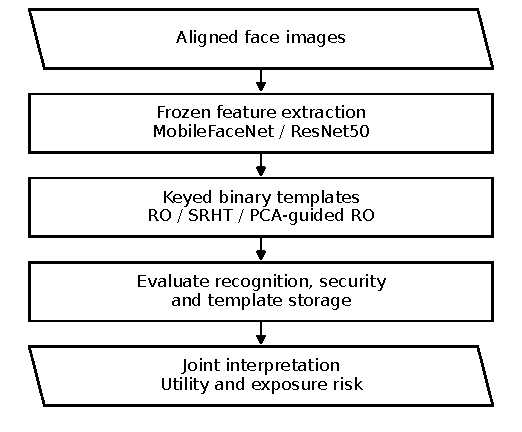
\includegraphics[width=\columnwidth]{methodology.pdf}
\caption{Overview of the evaluation: matched feature extraction and keyed protection feed recognition, security, and template-storage analyses.}
\label{fig:methodology}
\fignote{The workflow links repeated-exposure security with template-storage accounting; device performance is outside the measured scope.}
\end{figure}


Let $I$ denote an aligned facial image, $f_\theta$ a frozen encoder, $d_0=512$ the raw feature dimension, $d$ the projection-input dimension, and $m$ the protected length. The normalized feature and protected representation are
\begin{equation}
 x=\frac{f_\theta(I)}{\|f_\theta(I)\|_2},\qquad z=g(x)\in\mathbb S^{d-1},
\end{equation}
where $\mathbb S^{d-1}$ is the unit sphere. The operator $\unit(u)=u/\|u\|_2$ applies to nonzero vectors. Indices $k$ and $q$ identify historical and fresh keys, respectively; $K$ counts exposed historical records, not identities. In the inversion experiment, all $K$ records encode the same source photograph. A second photograph of the same identity supplies the cross-image enrollment reference. This distinction separates renewal exposure from variation across capture sessions.



For either encoder, $g$ is the identity map or a normalized PCA mapping. Applying the keyed matrix $W_k\in\mathbb{R}^{d\times m}$ and retaining its projection signs gives the $m$-bit template:
\begin{equation}
 b_k(x)=\mathbb{I}[W_k^\top g(x)\geq0]\in\{0,1\}^{m}.
\end{equation}
Protected templates are compared by their fraction of agreeing bits:
\begin{equation}
 s_H(b,b')=1-\frac{1}{m}\sum_{j=1}^{m}(b_j\oplus b'_j).
\end{equation}
A protected comparison is accepted when $s_H\geq\tau$; raw embeddings are compared by cosine similarity. TAR measures acceptance among genuine comparisons, FAR among impostor comparisons, and ASR among attack submissions. The validation FAR target controls threshold calibration and must be distinguished from the FAR subsequently observed on test data.


For RO, a seeded Gaussian matrix admits the thin factorization
\begin{equation}
 G_k=Q_kR_k,\quad Q_k^\top Q_k=I_m,\quad W_k=Q_k.
\label{eq:ro}
\end{equation}
The frozen QR sign convention and matrix shape are retained. CFP E06--E07 factorizes a square matrix and selects its first $m$ columns; the original LFW implementation uses reduced QR. These constructions share orthogonality but need not generate the same seeded bits.

For SRHT, let $D_k$ be a diagonal matrix of keyed Rademacher signs, $H_d$ the normalized Hadamard matrix, and $S_k\in\{0,1\}^{d\times m}$ select distinct keyed coordinates. Then
\begin{equation}
 W_k=D_kH_d^\top S_k,\quad
 W_k^\top z=S_k^\top H_dD_kz.
\label{eq:srht}
\end{equation}
Here $H_d^\top H_d=I_d$ and the tested dimensions admit a Hadamard transform. A positive scalar multiplier does not change the sign template. The stored implementation convention, including coordinate ordering, determines the reproducible bits.

PCA-guided RO first estimates a mean $\mu$ and leading eigenvectors from the permitted fitting set $\mathcal C$:
\begin{align}
 \mu&=|\mathcal C|^{-1}\sum_{i\in\mathcal C}x_i,\\
 C&=|\mathcal C|^{-1}\sum_{i\in\mathcal C}(x_i-\mu)(x_i-\mu)^\top,\\
 CU_d&=U_d\Lambda_d,\qquad g(x)=\unit\!\left(U_d^\top(x-\mu)\right).
\label{eq:pca}
\end{align}
No whitening is applied. The dimension is $d=256$ for 128-bit templates and $d=512$ for CFP 512-bit templates. The latter is a full centered rotation rather than dimensionality reduction. Original attack protocols fit PCA on separate calibration identities; the LFW encoder comparison uses the fold-specific exclusions in Section~\ref{sec:setup}.


For $N$ stored references and float32 raw features, template-only storage and its reduction are
\begin{align}
 B_m&=\lceil m/8\rceil,\quad B_{\rm raw}=4d_0=2048,\\
 S_m(N)&=NB_m,\quad R_m=B_{\rm raw}/B_m,\\
 \eta_m&=100\left(1-B_m/B_{\rm raw}\right)\%.
\label{eq:storage}
\end{align}
The tested lengths are byte-aligned. A useful system-level accounting identity is
\begin{equation}
 S_{\rm total}=S_m(N)+S_{\rm models}+S_{\rm operators}
 +S_{\rm keys}+S_{\rm metadata}.
\end{equation}
Only $S_m(N)$ is quantified here. Dense projection requires $O(dm)$ arithmetic operations; a fast Hadamard implementation requires $O(d\log d)$ before coordinate selection. PCA adds a dense $d_0$-to-$d$ mapping, and packed matching needs $O(\lceil m/w\rceil)$ XOR/popcount operations for word width $w$. These are algorithmic operation counts, not measured latency or energy, and they do not establish that the executed implementation achieves the fast-transform bound.

MobileFaceNet and binary Hamming matching were selected with constrained devices in mind. This paper compares their template-storage choices using measured TAR, FAR, linkage, and ASR. The experiments do not measure on-device response time, peak memory, power, or energy. Public kiosks and smart gadgets are motivating deployment examples, not evaluated platforms. This boundary prevents a smaller template from being mistaken for a demonstrated reduction in total system cost.


Table~\ref{tab:threat} separates the attacker assumptions. The linkage attacker receives $K$ older bit strings and a query template under another key. It does not receive projection operators or the target's raw embedding. The inversion attacker also receives the old operators and template/embedding pairs from other training identities. The algorithm and public PCA model are known. The fresh query operator is hidden during reconstruction and applied only by the verifier.

\begin{table*}[t]
\caption{Attacker access and the security question tested.}
\label{tab:threat}\centering\small
\begin{tabularx}{\textwidth}{@{}>{\raggedright\arraybackslash}p{2.3cm}>{\raggedright\arraybackslash}p{4.5cm}>{\raggedright\arraybackslash}X@{}}\toprule
Experiment & Available information or input & Interpretation \\\midrule
Verification utility & Legitimate same-key reference and probe & Recognition at a separately calibrated threshold.\\
Revoked replay & Unchanged old bit string; new-key reference & Accidental acceptance after renewal with metadata bypassed.\\
Template-only linkage & Historical bit strings and fresh query template & Learned same-identity discrimination without operators.\\
Embedding inversion & Old bit strings, old operators, auxiliary training pairs & Digital embedding-input acceptance under an unexposed key.\\
Image/camera attack & Would require image synthesis or sensor presentation & Outside the experiments; no corresponding success claim.\\\bottomrule
\end{tabularx}
\tabnote{Each test uses the stated attacker information; image and camera attacks are outside scope.}
\end{table*}

A system may reject an outdated reference through a version check before evaluating its similarity. To isolate matching behavior, the replay test bypasses that check and submits the old bits unchanged to the renewed matcher. Inversion instead submits an estimated embedding, which the verifier transforms using its fresh key. Success in this latter test presupposes access to a digital embedding-input interface.


With signed bits $y_k=2b_k-1$, the analytical estimate averages backprojections from the exposed keys:
\begin{equation}
 v_K=\frac{1}{K}\sum_{k\in\mathcal{E}_K}W_k y_k,
 \qquad \hat z_{\mathrm{an}}=\unit(v_K).
\end{equation}
The set $\mathcal{E}_K$ contains exposed keys only. A calibrated version fits one scale and one offset per coordinate using training identities:
\begin{equation}
 \hat z_{\mathrm{cal}}=\unit(a\odot v_K+c).
\end{equation}
For coordinate $j$, the fitted values are $a_j=\operatorname{Cov}(v_j,z_j)/\max(\operatorname{Var}(v_j),10^{-8})$ and $c_j=\bar z_j-a_j\bar v_j$. No nonlinear decoder or target-specific fitting is used. A PCA estimate is mapped back through the public basis and mean. The inverse uses a projected magnitude estimated from training data: the mean for CFP and the median for LFW. It does not use the unknown target magnitude.

Let $x_a$ be the exposed photograph and $x_b$ a different enrollment photograph of the same person. The main attack measure is acceptance of the reconstruction against $x_b$ under a fresh key:
\begin{equation}
 \ASR=\frac{1}{N}\sum_{i=1}^{N}\mathbb{I}
 [s_H(b_{q_i}(\hat x_i),b_{q_i}(x_{b,i}))\geq\tau_{q_i}].
\end{equation}
Results average the prescribed identities, trials, and splits. Using another photograph tests whether recovery remains useful beyond the exposed image. Additional measures are acceptance against that exposed image, cosine similarity to its embedding, and acceptance by the raw cosine matcher at its own threshold. Uninformed submissions use the normalized mean training embedding in LFW and embeddings of non-target training identities in CFP. These controls are distinct from the impostor comparisons used to estimate FAR.



Stacking the compromised operators yields
\begin{equation}
 A_K=\begin{bmatrix}W_{k_1}^\top\\\vdots\\W_{k_K}^\top\end{bmatrix},
 \quad y_K=\begin{bmatrix}y_{k_1}\\\vdots\\y_{k_K}\end{bmatrix},
 \quad y_K=\operatorname{sign}(A_Kz).
\end{equation}
Each nonzero signed measurement restricts $z$ to a hemisphere. A closed relaxation of the consistent directions is
\begin{equation}
 \mathcal F_K=\{u\in\mathbb S^{d-1}:\operatorname{diag}(y_K)A_Ku\succeq0\}.
\label{eq:feasible}
\end{equation}
Negative bits use a strict inequality under the implementation's zero-tie convention; the closed set includes its boundary. With the nested exposure schedule, $\mathcal F_{K+1}\subseteq\mathcal F_K$. Additional signs cannot enlarge this feasible set, although redundant measurements need not shrink it. This geometric observation does not guarantee monotone acceptance for a finite-data reconstruction algorithm.

For an idealized independent Gaussian row $a\sim\mathcal N(0,I_d)$ and fixed unit $z$,
\begin{equation}
 \mathbb E[a\,\operatorname{sign}(a^\top z)]=\sqrt{2/\pi}\,z.
\label{eq:gaussian}
\end{equation}
To see this, write $a=tz+a_\perp$, where $t\sim\mathcal N(0,1)$ and $a_\perp$ is independent with zero mean. The expectation becomes $\mathbb E|t|z$. This identity motivates signed backprojection and is consistent with one-bit recovery theory~\cite{plan2013,jacques2013}. The experiment uses correlated orthogonal or structured rows and non-Gaussian face features; therefore, this illustration is not a recovery theorem for RO, SRHT, or PCA-guided RO. Likewise, $Km$ is a count of binary observations, not an estimate of independent information bits or cryptographic security strength.


Coordinate calibration uses ordinary least-squares slopes and intercepts estimated from auxiliary training examples. Ignoring the numerical variance floor, the fit for coordinate $j$ minimizes
\begin{equation}
 \min_{a_j,c_j}\sum_{i\in\mathcal T}
 \left[z_{ij}-(a_jv_{K,ij}+c_j)\right]^2.
\end{equation}
The $10^{-8}$ floor stabilizes nearly constant coordinates and is not a tuned ridge penalty. For PCA protection, lifting back to the raw feature space uses
\begin{equation}
 \hat x=\unit(\mu+\rho_{\mathcal T}U_d\hat z),
\label{eq:lift}
\end{equation}
where $\rho_{\mathcal T}$ is the training-only mean projected norm in CFP and median projected norm in LFW. For RO and SRHT, $\hat x=\hat z$. Source reconstruction quality is $c_{\rm src}=\hat x^\top x_a$; cross-image quality is $c_{\rm cross}=\hat x^\top x_b$. Neither quantity determines acceptance without the fresh transformation and threshold.

The attack's information set is $\mathcal I_K=\{(b_k(x_a),W_k):k\in\mathcal E_K\}$ plus the public preprocessing and auxiliary training information. Reconstruction has the form $\hat x=\mathcal A(\mathcal I_K)$, with $q\notin\mathcal E_K$. The verifier alone computes $b_q(\hat x)$ and compares it with $b_q(x_b)$. Thus, concealing the fresh operator is an explicit experimental constraint; it does not erase constraints already disclosed by the historical operators.


For genuine scores $\mathcal G$ and impostor scores $\mathcal J$, the empirical rates at threshold $\tau$ are
\begin{align}
 \widehat{\TAR}(\tau)&=|\mathcal G|^{-1}\sum_{s\in\mathcal G}\mathbb I[s\geq\tau],\\
 \widehat{\FAR}(\tau)&=|\mathcal J|^{-1}\sum_{s\in\mathcal J}\mathbb I[s\geq\tau].
\end{align}
Protected scores lie on the grid $\{0,1/m,\ldots,1\}$. The frozen validation rule selects the least restrictive attainable acceptance set containing at most $\lfloor\alpha|\mathcal J_{\rm val}|\rfloor$ impostor scores. A threshold just above a tied boundary excludes the entire tied group. Consequently, calibration at target $\alpha$ need not achieve equality, and observed test FAR is a separate quantity.

For an old-to-new key transition, unchanged-template replay is
\begin{equation}
 \widehat R_{k\to q}=\frac1n\sum_{i=1}^n
 \mathbb I[s_H(b_k(x_{a,i}),b_q(x_{b,i}))\geq\tau_q].
\end{equation}
This definition follows the image pairing prescribed by the replay protocol; it differs from fresh-key ASR because no reconstruction is submitted. For learned linkage score $\ell$, ROC AUC estimates
\begin{equation}
 \Pr(\ell_{\rm same}>\ell_{\rm different})+
 \tfrac12\Pr(\ell_{\rm same}=\ell_{\rm different}).
\end{equation}
AUC is score-specific. Direction-aware basic diagnostics use $\max(\mathrm{AUC},1-\mathrm{AUC})$; learned linkage retains the trained score direction. Neither chance-level AUC nor a low replay rate establishes irreversibility.

\section{Experimental Setup}\label{sec:setup}


LFW preprocessing uses SCRFD-500MF~\cite{guo2021scrfd}, detection threshold 0.50, and $640\times640$ input. The largest detected face is aligned to $112\times112$ using five landmarks. The fixed pretrained \texttt{w600k\_mbf} encoder produces the normalized 512-dimensional vector. The 6000 official pairs use 7701 distinct images. Extraction succeeds for 7682 images; 19 failures affect 35 pairs. Full-pipeline results count these failures as rejections. Matcher-only results use the 5965 pairs for which both embeddings exist.

CFP has 500 identities, each with ten frontal and four profile images~\cite{sengupta2016cfp}. The official CFP-FP protocol contains 7000 pairs, half genuine and half impostor. Its aligned-bin baseline includes all 14,000 pair sides and 5890 unique encoded crops, which are passed directly to the encoder. Earlier raw-image detection attempts achieved only 5.73\%, 47.66\%, and 49.70\% coverage. They failed the coverage requirement and are excluded from recognition reporting. The datasets thus use the same baseline encoder but different preprocessing paths.

Official thresholds are selected on nine pair folds and tested on the remaining fold. The CFP length study uses ten RO keys at 64, 128, 256, and 512 bits. Its projections are generated separately for each length, unlike the nested-column construction in CFP E06--E07. The CFP replay study tests all 90 directed changes among ten keys and 3500 genuine pairs per change. Its 315,000 decisions reuse people, images, and keys and are not independent observations.


Table~\ref{tab:protocol} gives the custom attack partitions. LFW PCA calibration uses one image from each of 1024 identities excluded from evaluation. The evaluation pool contains 3250 identities and 6658 usable images. Verification uses 300 genuine and 300 impostor pairs per fold, with at most ten genuine pairs per identity. E07 selects 1200 identities, each with two different images, balanced across ten folds. Calibration and threshold selection use the other nine identity folds. Twenty base keys support ten held-out-query trials, with nested exposure counts $K\in\{1,2,5,10\}$.

The screened CFP pool contains 5704 crops from all 500 identities. Each of three seeded partitions assigns 100 identities to PCA calibration, 250 to attacker training, 75 to validation, and 75 to testing. These sets are disjoint within a partition. Across partitions they overlap, and the test sets cover 195 distinct identities. Partition seeds are 2026092201--2026092203; key seeds are 24001--24020. Each query key is excluded from the next ten exposed keys in the rotating schedule. Inversion uses one deterministically selected frontal image and one profile image per identity, tested in both directions. Genuine utility uses the larger frozen E06 validation/test pair lists rather than only these attack images.

\begin{table*}[t]
\caption{Original MobileFaceNet attack protocols.}
\label{tab:protocol}\centering\small
\begin{tabularx}{\textwidth}{@{}>{\raggedright\arraybackslash}p{3.2cm}>{\raggedright\arraybackslash}X>{\raggedright\arraybackslash}X@{}}\toprule
Item & LFW E07 & CFP E06--E07 screened subset\\\midrule
Preprocessing & SCRFD detection and alignment & Already aligned bin crops\\
Encoder / input dimension & Frozen MobileFaceNet / 512 & Frozen MobileFaceNet / 512\\
Template lengths & 128 bits & 128 and 512 bits\\
PCA calibration & 1024 identities, one image each & 100 identities per partition\\
Attack partition & Ten identity folds, training on other nine & 250 train / 75 validation / 75 test identities\\
Attack targets & 1200 identities, two images each & 75 identities per split, one image per pose\\
Repeated evaluations & Ten query-key trials & Three overlapping splits; twenty query-key rotations\\
Unique test identities & 1200 & 195 across repetitions\\
Threshold source & Other nine identity folds & Validation identities only\\
Exposure counts & $K=1,2,5,10$ & $K=1,2,5,10$\\\bottomrule
\end{tabularx}
\tabnote{Training and test identities are separate within each protocol; CFP repetitions overlap.}
\end{table*}


The exact frozen QA01 bin was recovered and checked against its SHA-256 digest. Hashes connect all 14,000 pair-side rows to the cached crops. The audit also checks 7000 source-file hashes and decoded RGB hashes for 5901 mapped source references. Some references contain identical image data, so their count exceeds the 5890 unique encoded crops.

Among the 5704 retained crops, 4295 pass the strict SIFT/affine check, 1380 have post-hoc overlap-only support, and three have post-hoc ECC registration support. The researcher visually reviewed the remaining 26 flagged cases and marked all as \texttt{SAME\_SOURCE}. This review changed neither the mapping nor the subset. The original 186 excluded crops remain excluded. The review resolves the flagged correspondences but is not independent certification of every identity label.

The correspondence controls comprise 500 images of different people and 500 alternative photographs of the same people. Neither control group passes the strict or overlap rules. This is useful supporting evidence, but the sample size, absence of a separate ECC negative-control study, post-hoc checks, and single reviewer limit the audit's strength. These screened attack data are retained separately from the official benchmark.


Linkage features include per-bit agreement, sorted cross-key Hamming similarities, and their mean, standard deviation, minimum, maximum, median, and range. A logistic-regression model with standardized features is fitted using training identities only. CFP uses $C=1$ and chooses the balanced-accuracy threshold on validation identities. LFW uses training and testing across identity folds. ROC AUC evaluates score ranking without requiring a binary threshold. Basic cross-key diagnostics use direction-aware AUC; learned attacks use the trained score direction.

The main matcher threshold targets FAR $\alpha=10^{-3}$ using non-test impostor scores. For CFP, sorted validation scores allow at most $\lfloor\alpha n\rfloor$ false accepts. The \texttt{nextafter} operation places the threshold just above the boundary score and handles ties conservatively. Test FAR is then measured separately. The original CFP sensitivity study repeats this rule at $\alpha\in\{10^{-4},5\!\times\!10^{-4},10^{-3},5\!\times\!10^{-3},10^{-2}\}$ without selecting thresholds from test labels. Frozen E06 scores reproduce the original operating point and avoid changes in template bits caused by cross-platform QR arithmetic.


Uncertainty in E07 is estimated from 2000 bootstrap draws of test identities. A sampled identity has a common weight across every key, direction, repetition, and method in which it appears. Weighted outcomes are computed within each split or fold before averaging those splits or folds equally. Applying the same draw to both sides of a paired contrast preserves the dependence created by repeated evaluation of the same person.

The percentile intervals describe variation across tested identities with the fitted models, PCA, selected images, keys, partitions, and thresholds fixed. They do not include refitting uncertainty, adjust for multiple comparisons, or provide population-wide guarantees. For CFP utility, genuine pairs use identity weights and impostor pairs use the product of the two identity weights. Earlier intervals across keys instead describe key variation. A matched threshold sweep for the original LFW attack study is unavailable because the retained files lack the full calibration-score cache.


Let $r_{i,s,c}$ be the acceptance fraction for identity $i$ in split or fold $s$ and configuration $c$, after averaging its prescribed repeated trials. When per-identity trial counts are equal, the reported estimator is
\begin{equation}
 \hat\theta_c=\frac1S\sum_{s=1}^S\frac1{n_s}\sum_{i\in\mathcal U_s}r_{i,s,c}.
\end{equation}
More generally, the implementation uses sample-weighted rates within each split, then gives splits equal weight. A bootstrap draw assigns global multiplicities
\begin{equation}
 (w_1^{(b)},\ldots,w_U^{(b)})\sim
 \operatorname{Multinomial}(U;1/U,\ldots,1/U).
\end{equation}
For trial outcome $Y_{t,c}$ and trial identity $i(t)$, its split contribution becomes
\begin{equation}
 \hat\theta_{s,c}^{(b)}=
 \frac{\sum_{t\in\mathcal T_s}w_{i(t)}^{(b)}Y_{t,c}}
 {\sum_{t\in\mathcal T_s}w_{i(t)}^{(b)}}.
\label{eq:bootstrap}
\end{equation}
An identity retains its sampled multiplicity across overlapping CFP partitions, keys, and directions. Genuine pairs receive the identity weight; an impostor pair between $i$ and $j$ receives $w_i^{(b)}w_j^{(b)}$. The 2.5th and 97.5th percentiles of the 2000 replicate estimates form the empirical 95\% interval. Retaining shared weights accounts for repeated observations more faithfully than an analysis that treats each decision as an independent Bernoulli trial.

Paired contrasts reuse the same draw on both sides:
\begin{align}
 \Delta_{\rm enc}^{(b)}&=\hat\theta_{\rm R50}^{(b)}-\hat\theta_{\rm MBF}^{(b)},\\
 \Delta_K^{(b)}&=\hat\theta_{K=10}^{(b)}-\hat\theta_{K=1}^{(b)}.
\end{align}
Contrasts in rate metrics are reported as $100\Delta$ percentage points. Non-overlap of two marginal intervals is not used as a substitute for a paired contrast. All intervals are pointwise and conditional on fitted models, partitions, selected images, keys, and validation thresholds; they do not account for model refitting or multiplicity. A degenerate empirical interval is not evidence of population certainty.




The second frozen checkpoint, InsightFace \texttt{w600k\_r50} trained with ArcFace~\cite{arcface}, tests whether the main finding occurs with another encoder. Both checkpoints output normalized 512-dimensional embeddings. The CFP replication uses identical aligned crops, the same screened subset, identity partitions, key schedule, and template lengths. PCA, reconstruction calibration, linkage models, and matching thresholds are fitted separately for each encoder using the prescribed partitions. ResNet50 serves as an encoder comparison, with no claim that its device cost matches MobileFaceNet. The comparison holds inputs and evaluation rules fixed, but does not isolate architecture from training data or loss. It does not match the encoders at exactly equal genuine TAR.

The LFW extension uses the original 6000 official pairs and ten folds. All 7701 image records are checked against the frozen MobileFaceNet extraction before ResNet50 receives the same aligned crops. Original raw and RO MobileFaceNet fold counts and packed templates are reproduced. Five fixed keys are used at 128 bits. SRHT uses new, recorded comparison keys. For PCA-guided RO, each fold has a separate 256-component PCA fitted to unique valid images from the other nine folds after excluding every identity present in the held-out fold. Official folds can share identities for threshold estimation; this is not the identity-disjoint LFW attack protocol. No second-encoder LFW attack result is claimed.


The CFP encoder replication uses three validation-FAR targets, $10^{-4}$, $10^{-3}$, and $10^{-2}$, and a descriptive sweep of discrete matching thresholds. Its 2000-replicate identity bootstrap follows the same global identity-weighting principle. All thresholds and fitted models remain fixed during resampling. The original CFP baseline and the encoder replication retain their own result tables; small differences between their runs are not pooled or silently replaced.

\section{Results}\label{sec:results}
We first report the original MobileFaceNet experiments, followed by the matched encoder replication. Unless stated otherwise, thresholds use a 0.1\% training or validation FAR target, with test FAR measured separately. Rates are expressed as percentages and their differences as percentage points; AUC and cosine similarity are unitless.


Table~\ref{tab:official} reports official-pair verification at a training FAR target of 0.1\%. Protected results average five LFW keys or ten CFP keys. On LFW, matcher-only TAR is 98.66\% for raw embeddings and 82.99\% for 128-bit RO. On CFP-FP, the raw baseline is 87.71\%, while RO TAR is 35.93\% at 128 bits and 80.50\% at 512 bits. The compact 128-bit representation therefore loses much more genuine acceptance in the frontal-to-profile setting.

\begin{table}[t]
\caption{Original MobileFaceNet verification on official pairs.}
\label{tab:official}\centering\small
\begin{tabular}{@{}llrrr@{}}\toprule
Dataset & Representation & TAR (\%) & FAR (\%) & Bytes\\\midrule
LFW & Raw 512-D & 98.66 & 0.101 & 2048\\
LFW & RO 128-bit & 82.99 & 0.094 & 16\\
CFP-FP & Raw 512-D & 87.71 & 0.143 & 2048\\
CFP-FP & RO 64-bit & 14.56 & 0.077 & 8\\
CFP-FP & RO 128-bit & 35.93 & 0.103 & 16\\
CFP-FP & RO 256-bit & 61.49 & 0.129 & 32\\
CFP-FP & RO 512-bit & 80.50 & 0.106 & 64\\\bottomrule
\end{tabular}
\tabnote{Official-pair rates use a 0.1\% training FAR target; LFW results are matcher-only.}
\end{table}

Across the CFP length study, TAR increases from 14.56\% at 64 bits to 80.50\% at 512 bits, leaving a 7.21-percentage-point gap to the raw baseline. The longer representation is consequently included in the attack evaluation: restricting that evaluation to short templates would assess protection at a substantially weaker genuine operating point.

When LFW detection failures count as rejections, full-pipeline TAR is 98.03\% for raw embeddings and 82.47\% for 128-bit RO. These values differ from the matcher-only rates in Table~\ref{tab:official}. CFP uses supplied aligned crops, so complete crop coverage does not demonstrate successful detection on its raw photographs.


Table~\ref{tab:storage} connects template size to the edge motivation. A 128-bit template needs 16 bytes, saving 99.22\% of the raw 2048-byte payload. A 512-bit template needs 64 bytes, saving 96.88\%. Equivalently, the payloads are 128 times and 32 times smaller than the raw embedding. These savings follow directly from the representation sizes and apply to each tested family at the stated length.

\begin{table}[t]
\caption{Packed template payload relative to a raw embedding.}
\label{tab:storage}\centering\small
\begin{tabular}{@{}lrrr@{}}\toprule
Representation & Bytes & Reduction & Saved (\%)\\\midrule
Raw 512-D float32 & 2048 & $1\times$ & 0.00\\
Protected 128-bit & 16 & $128\times$ & 99.22\\
Protected 512-bit & 64 & $32\times$ & 96.88\\\bottomrule
\end{tabular}
\tabnote{Savings cover packed templates only; model, operator, key, and metadata costs are excluded.}
\end{table}

For $N$ enrolled references, the template payload is $2048N$, $16N$, or $64N$ bytes. Increasing CFP RO payload from 16 to 64 bytes raises official TAR from 35.93\% to 80.50\%, but the custom experiments below also reveal greater reconstruction risk. The storage advantage must therefore be weighed against both recognition and exposure outcomes.

Figure~\ref{fig:storage-scaling} expresses the same deterministic payload accounting over database size. It isolates the template component and therefore does not measure full application memory.
\begin{figure}[!tb]
\centering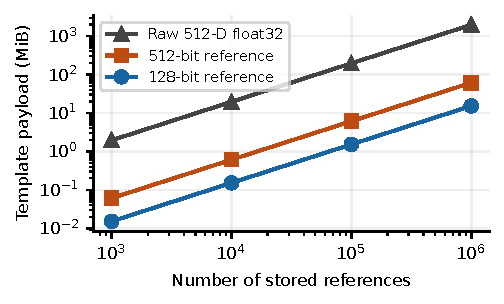
\includegraphics[width=\columnwidth]{storage_scaling.pdf}
\caption{Calculated template-only storage as the number of enrolled references grows. Both axes are logarithmic; one MiB is $2^{20}$ bytes.}
\label{fig:storage-scaling}\fignote{Curves exclude model weights, working memory, keys, operators, and metadata.}
\end{figure}


Table~\ref{tab:replay} tests whether unchanged old bits are accepted after a key change, with version checks bypassed. CFP accepts 106 of 315,000 decisions at 128 bits and 10 at 512 bits. These trials reuse subjects and keys, so the counts describe the test schedule rather than independent risk observations. Recalculation from the cache reproduces the saved scores, thresholds, and decisions.

\begin{table}[t]
\caption{Acceptance of unchanged old templates after renewal.}
\label{tab:replay}\centering\small
\begin{tabular}{@{}lrrr@{}}\toprule
Dataset / bits & Accepted / trials & Rate (\%) & Worst (\%)\\\midrule
LFW / 128 & 28 / 59,620 & 0.04696 & 0.101\\
CFP-FP / 128 & 106 / 315,000 & 0.03365 & 0.2857\\
CFP-FP / 512 & 10 / 315,000 & 0.00317 & 0.0571\\\bottomrule
\end{tabular}
\tabnote{Unchanged old templates rarely pass the renewed matcher; repeated trials are dependent.}
\end{table}

The LFW version gate rejects every revoked version in its test. Genuine acceptance can still vary after renewal: TAR differs by up to 5.64 percentage points between two keys. Basic cross-key Hamming scores give pooled AUC 0.5020 on LFW and 0.5010/0.5027 on CFP at 128/512 bits, close to chance on average. The worst individual key-pair AUC is 0.5256 on LFW and 0.5454 on CFP at 512 bits. The CFP diagnostic compares images without disjoint test-identity partitions and should be read within that scope.


The learned LFW attack finds a small same-person signal. In the original multiple-exposure test, AUC changes from 0.5558 at one exposure to 0.5583 at ten. Rebuilding pairs with separate training and test identities gives 0.5580 and 0.5595. A signal therefore remains for unseen people. Since pair construction also changed, identity separation alone cannot explain the difference between the two tests.

Table~\ref{tab:linkage} gives E06 means for each dataset's own identity-disjoint protocol. With ten exposures, CFP AUC is 0.5323--0.5377 at 128 bits and 0.5629--0.5667 at 512 bits. The longer template improves genuine matching but gives this attacker a stronger ranking signal. Small differences among the projection methods should not be confused with the larger change in threat model when old operators are revealed.

\begin{table}[t]
\caption{Template-only linkage AUC at ten exposures.}
\label{tab:linkage}\centering\small
\begin{tabular}{@{}lrrr@{}}\toprule
Method & LFW 128 & CFP 128 & CFP 512\\\midrule
RO & 0.5594 & 0.5328 & 0.5667\\
SRHT & 0.5577 & 0.5323 & 0.5629\\
PCA-guided RO & 0.5687 & 0.5377 & 0.5643\\\bottomrule
\end{tabular}
\tabnote{AUC describes template-only identity linkage at ten exposures; chance ranking is 0.5.}
\end{table}


Table~\ref{tab:attackutility} gives legitimate utility for the custom E07 protocols at a training/validation FAR target of 0.1\%. In this original custom protocol, the screened CFP raw baseline has TAR 91.47\% and observed FAR 0.325\%. Its images, pair lists, partitions, and thresholds differ from the official benchmark. Attack rates must therefore be compared with this custom protocol's utility, not substituted into the official results.

\begin{table}[t]
\caption{Genuine utility in the original custom attack protocols.}
\label{tab:attackutility}\centering\small
\begin{tabular}{@{}llrr@{}}\toprule
Protocol & Method & TAR (\%) & FAR (\%)\\\midrule
LFW, 128 bits & RO & 83.34 & 0.077\\
 & SRHT & 82.00 & 0.087\\
 & PCA-guided RO & 84.89 & 0.087\\
CFP screened, 128 & RO & 39.33 & 0.134\\
 & SRHT & 37.76 & 0.113\\
 & PCA-guided RO & 43.50 & 0.115\\
CFP screened, 512 & RO & 82.52 & 0.172\\
 & SRHT & 81.95 & 0.167\\
 & PCA-guided RO & 82.38 & 0.200\\\bottomrule
\end{tabular}
\tabnote{These custom-protocol rates are the genuine operating points for the inversion study.}
\end{table}

\begin{table*}[t]
\caption{Original MobileFaceNet calibrated inversion: fresh-key attack success and reconstruction quality.}
\label{tab:inversion}\centering\small
\begin{tabular}{@{}lrlrrrr@{}}\toprule
Protocol & Bits & Method & Fresh ASR, $K=1$ & Fresh ASR, $K=10$ [95\% CI] & Cosine & Raw ASR\\\midrule
% BEGIN GENERATED ATTACK ROWS
LFW & 128 & RO & 9.13 & 66.63 [64.96, 68.31] & 0.8103 & 97.22 \\
LFW & 128 & SRHT & 8.39 & 64.53 [62.86, 66.22] & 0.8096 & 97.30 \\
LFW & 128 & PCA-guided RO & 34.50 & 80.96 [79.47, 82.44] & 0.8635 & 97.53 \\
CFP screened & 128 & RO & 2.01 & 19.66 [17.23, 22.38] & 0.8105 & 84.22 \\
CFP screened & 128 & SRHT & 1.93 & 18.84 [16.42, 21.41] & 0.8099 & 84.28 \\
CFP screened & 128 & PCA-guided RO & 7.86 & 32.94 [29.35, 36.96] & 0.8593 & 86.32 \\
CFP screened & 512 & RO & 63.27 & 78.02 [73.38, 82.52] & 0.9725 & 88.22 \\
CFP screened & 512 & SRHT & 62.64 & 77.52 [72.95, 82.10] & 0.9726 & 88.09 \\
CFP screened & 512 & PCA-guided RO & 70.28 & 78.54 [73.89, 83.03] & 0.9809 & 88.72 \\
% END GENERATED ATTACK ROWS

\bottomrule
\end{tabular}
\tabnote{ASR values are percentages; brackets show conditional 95\% intervals for fresh-key ASR at ten exposures.}
\end{table*}

\begin{figure*}[!t]
\centering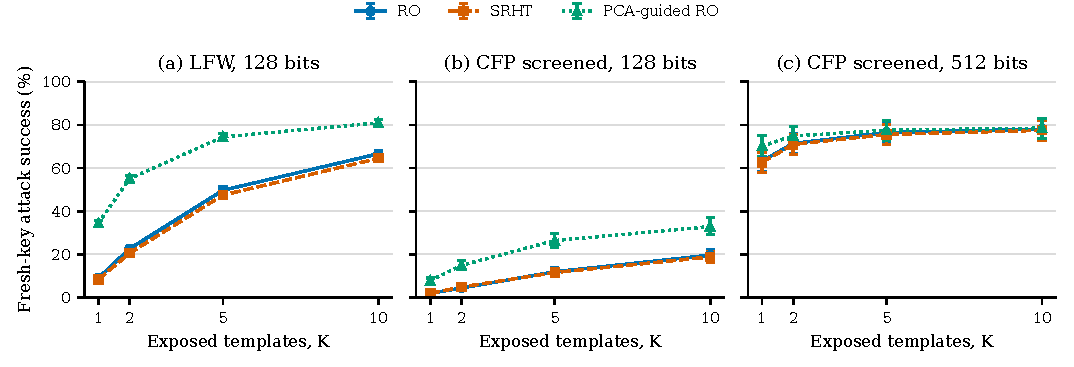
\includegraphics[width=\textwidth]{exposure.pdf}
\caption{Fresh-key attack success increases with exposure; error bars show conditional 95\% identity-bootstrap intervals.}
\label{fig:exposure}
\fignote{More exposed records provide useful reconstruction information in the tested configurations.}
\end{figure*}

\begin{figure*}[!t]
\centering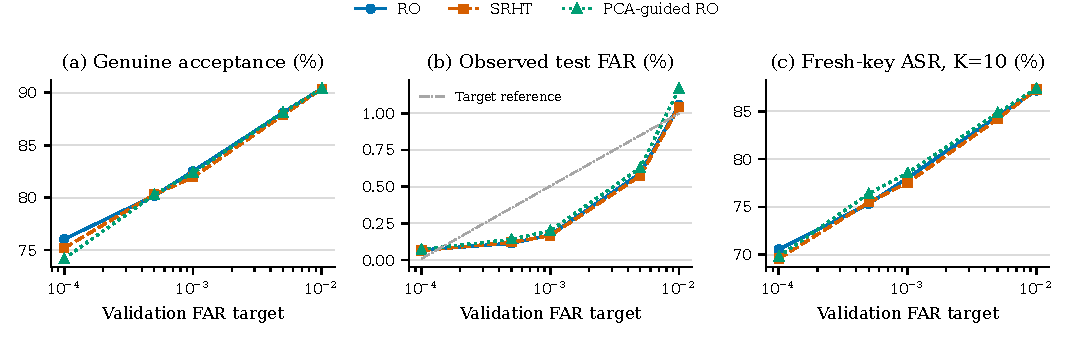
\includegraphics[width=\textwidth]{thresholds.pdf}
\caption{Stricter validation targets reduce genuine and attack acceptance on screened CFP at 512 bits.}
\label{fig:thresholds}
\fignote{Lower attack acceptance must be interpreted together with genuine-user rejection.}
\end{figure*}

Across the three projection methods, calibrated cross-image fresh-key ASR at ten exposures is 64.53--80.96\% on LFW at 128 bits, 18.84--32.94\% on screened CFP at 128 bits, and 77.52--78.54\% on screened CFP at 512 bits. The CFP attack pool contains 5704 crops from 500 identities before partitioning. These ranges describe the original run; the matched CFP encoder replication is reported separately below. Table~\ref{tab:inversion} reports ASR in percent; its brackets give conditional 95\% identity-bootstrap intervals from 2000 replicates. Cosine similarity and raw ASR are measured at $K=10$, with cosine taken against the exposed image.

Figure~\ref{fig:exposure} shows the exposure effect on a common vertical scale. In both result figures, blue solid lines with circles represent RO, orange dashed lines with squares represent SRHT, and green dotted lines with triangles represent PCA-guided RO. Exposure error bars show pointwise conditional 95\% intervals. LFW and CFP retain their separate protocols.

On LFW, ten-exposure ASR is 66.63\% for RO, 64.53\% for SRHT, and 80.96\% for PCA-guided RO. The corresponding uninformed rates are 0.53\%, 0.40\%, and 0.13\%. Acceptance against the exposed image is almost 100\%. Testing against a different photograph is therefore a more informative primary measure than reusing the source image.

At 128 bits on CFP, RO and SRHT recover the source embedding with cosine similarities 0.8105 and 0.8099, close to LFW's 0.8103 and 0.8096. Yet fresh-key cross-pose ASR is only 19.66\% and 18.84\%. PCA-guided RO gives cosine 0.8593 and ASR 32.94\%. This lower attack acceptance accompanies weak genuine cross-pose recognition. Under the separate raw-matcher threshold, reconstructed CFP embeddings reach 84.22--86.32\% ASR.

At 512 bits on CFP, cosine similarity reaches 0.9725, 0.9726, and 0.9809 for RO, SRHT, and PCA-guided RO. Their fresh-key ASRs are 78.02\% [73.38, 82.52], 77.52\% [72.95, 82.10], and 78.54\% [73.89, 83.03]. Uninformed rates are 0.08--0.16\%, while raw ASR is 88.09--88.72\%. The rare acceptance of unchanged old bits does not account for these newly reconstructed inputs.

Diagonal calibration is not necessary for substantial acceptance in the 512-bit CFP setting. At ten exposures, analytical backprojection reaches ASRs of 77.93\%, 77.33\%, and 78.06\% for RO, SRHT, and PCA-guided RO, respectively. Calibration provides only a small additional gain here. These results establish the measured risk with a simple estimator; they do not assess what a more complex decoder might recover.


All paired intervals for calibrated $K=10$ minus $K=1$ ASR lie above zero. The increases for RO, SRHT, and PCA-guided RO are 57.50, 56.13, and 46.46 percentage points on LFW; 17.64, 16.91, and 25.09 on CFP at 128 bits; and 14.76, 14.88, and 8.27 on CFP at 512 bits. The 512-bit increases are smaller because single-exposure ASR is already 62.64--70.28\%.

At ten exposures, the CFP 512-bit intervals overlap across methods. The source package includes paired method contrasts, but ranking protection from the point estimates alone is not justified. Under known-operator exposure, substantial attack acceptance occurs for all three projection families.


Figure~\ref{fig:thresholds} reports means over fixed keys and splits for screened CFP at 512 bits. The attack panel uses calibrated reconstruction with ten exposures. The gray dash-dot line in the FAR panel marks equality between test FAR and the validation target, expressed as percentages. For RO, tightening the target from $10^{-3}$ to $10^{-4}$ lowers TAR from 82.52\% to 76.04\% and ASR from 78.02\% to 70.56\%. Across methods, ASR remains 69.59--70.56\% at the tighter setting. At the looser $10^{-2}$ target, TAR is about 90.4\% and ASR is 87.17--87.38\%. Stricter matching reduces acceptance for both users and attackers but does not remove the observed risk.

Each validation split contains only 2105--2173 impostor comparisons. The $10^{-4}$ target allows no validation false accepts, yet test FAR is 0.0656--0.0736\%, above the nominal 0.01\%. This sample cannot establish a population FAR of $10^{-4}$. At the main 0.1\% target, CFP 512-bit test FAR is 0.167--0.200\%. Every operating point must therefore be interpreted with its observed FAR.




On official CFP-FP pairs, raw TAR increases from 87.71\% for MobileFaceNet to 94.89\% for ResNet50 at the 0.1\% training-FAR target. Both have observed test FAR 0.143\%. Table~\ref{tab:encoder-cfp} reports the separate screened-subset comparison. Protected TAR rises for every method and length: from \MbfSmallTar{} to \RnetSmallTar{} at 128 bits, and from \MbfLargeTar{} to \RnetLargeTar{} at 512 bits.

Higher utility does not remove the tested reconstruction vulnerability. At ten exposures, MobileFaceNet calibrated cross-image fresh-key ASR is \MbfSmallAsr{} at 128 bits and \MbfLargeAsr{} at 512 bits. The corresponding ResNet50 ranges are \RnetSmallAsr{} and \RnetLargeAsr{}. All six paired ResNet50-minus-MobileFaceNet ASR intervals lie above zero. These pointwise intervals resample the 195 unique test identities while retaining dependencies across overlapping splits and keys; they condition on the fitted models and thresholds. They do not establish that every stronger encoder is less secure.

Fresh-key acceptance and reconstruction cosine do not improve in parallel. For 128-bit RO and SRHT, exposed-image cosine stays near 0.81 with either encoder, although acceptance rises with ResNet50. All three 512-bit ResNet50 configurations also admit high acceptance. Thus, stronger genuine recognition cannot be taken as evidence that the protected representation better resists known-operator reconstruction.

Table~\ref{tab:encoder-lfw} gives the corresponding LFW recognition extension. Raw matcher-only TAR changes from 98.66\% to 99.03\%. At 128 bits, ResNet50 TAR is 92.28\% for RO, 92.10\% for SRHT, and 94.66\% for PCA-guided RO, compared with 82.99\%, 84.48\%, and 85.22\% for MobileFaceNet. These recognition results extend the utility comparison; they do not extend the LFW attack evidence.

\begin{table*}[t]
\caption{Matched encoder comparison on screened CFP. Rates are percentages; ASR differences are percentage points.}
\label{tab:encoder-cfp}\centering\footnotesize
\begin{tabular}{@{}rlrrrrr@{}}\toprule
Bits & Method & MBF TAR / FAR & R50 TAR / FAR & MBF ASR & R50 ASR & ASR difference [95\% CI]\\\midrule
128 & RO & 39.33 / 0.134 & 65.50 / 0.133 & 19.66 & 38.46 & 18.80 [16.68, 20.86]\\
128 & SRHT & 37.76 / 0.113 & 65.12 / 0.120 & 18.84 & 38.28 & 19.43 [17.03, 21.81]\\
128 & PCA-guided RO & 43.50 / 0.115 & 66.94 / 0.103 & 32.96 & 53.09 & 20.13 [17.74, 22.68]\\
512 & RO & 82.52 / 0.172 & 94.61 / 0.134 & 78.02 & 92.30 & 14.28 [11.13, 17.52]\\
512 & SRHT & 81.95 / 0.167 & 94.67 / 0.128 & 77.52 & 92.23 & 14.71 [11.67, 17.95]\\
512 & PCA-guided RO & 82.38 / 0.200 & 94.37 / 0.130 & 78.56 & 92.03 & 13.48 [10.34, 16.72]\\
\bottomrule\end{tabular}
\tabnote{MBF: MobileFaceNet; R50: ResNet50 ArcFace. Each encoder has a separate validation-only threshold targeting 0.1\% FAR. ASR is calibrated cross-image fresh-key acceptance at $K=10$. The fresh operator is hidden from reconstruction. Paired percentile intervals use 2000 identity resamples and condition on the fitted pipelines; they are pointwise and not multiplicity-adjusted. These replication runs remain separate from the original baseline tables.}
\end{table*}

\begin{table}[t]
\centering
\caption{LFW official-pair recognition: encoder comparison.}
\label{tab:encoder-lfw}
\small
\begin{tabular}{lrrrr}
\toprule
& \multicolumn{2}{c}{TAR (\%)} & \multicolumn{2}{c}{FAR (\%)} \\
Method & MBF & R50 & MBF & R50 \\
\midrule
Raw & 98.66 & 99.03 & 0.101 & 0.101 \\
RO & 82.99 & 92.28 & 0.094 & 0.080 \\
SRHT & 84.48 & 92.10 & 0.094 & 0.094 \\
PCA-guided RO & 85.22 & 94.66 & 0.087 & 0.094 \\
\bottomrule
\end{tabular}
\tabnote{Matcher-only evaluation uses 5965 valid pairs, with thresholds fitted on the other nine folds at a 0.1\% FAR target. Protected templates have 128 bits; rates average five fixed keys. MBF: MobileFaceNet; R50: ResNet50 ArcFace. The full 6000-pair operational results are retained in the evidence. Fold-specific PCA excludes held-out identities from fitting.}
\end{table}


\begin{figure*}[!t]
\centering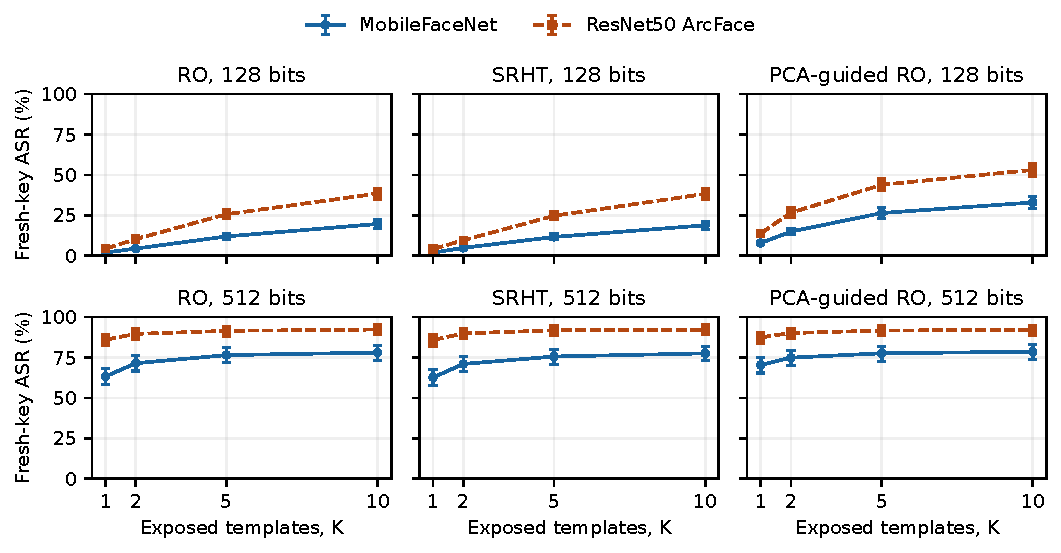
\includegraphics[width=0.92\textwidth]{encoder_exposure.pdf}
\caption{CFP encoder replication: calibrated cross-image fresh-key ASR over exposure count at 128 bits (top) and 512 bits (bottom). Error bars show pointwise conditional 95\% identity-bootstrap intervals. Both encoders use identical screened crops and exposure schedules, with separately fitted models and validation-only thresholds.}
\label{fig:encoder-exposure}
\fignote{The stronger recognition checkpoint still permits substantial fresh-key attack acceptance.}
\end{figure*}


Unchanged old CFP records continue to have low cross-image replay acceptance. Across the two encoders, three methods, and two directions, mean transition rates are approximately 0.038--0.076\% at 128 bits and 0.004--0.013\% at 512 bits. Template-only linkage with ten records has trained-score AUC 0.530--0.542 at 128 bits and 0.559--0.567 at 512 bits. These descriptive outcomes concern the tested classifier and fixed key schedule; they do not prove unlinkability or resistance to a stronger attacker.

The replication reports conditional intervals at validation-FAR targets $10^{-4}$, $10^{-3}$, and $10^{-2}$, together with a descriptive threshold sweep and measured test FAR alongside TAR and ASR. Complete exposure curves, paired contrasts, and threshold plots are retained in the accompanying results. Lower attack acceptance under stricter matching must be read alongside increased genuine rejection. The hidden fresh operator and digital embedding-input interface remain unchanged.


Figures~\ref{fig:cfp-recognition} and~\ref{fig:lfw-recognition} present recognition separately for the screened CFP protocol and official LFW pairs. CFP intervals quantify conditional identity variation; LFW error bars describe variation across five fixed keys and are not confidence intervals. The two uncertainty summaries must not be conflated.

Figure~\ref{fig:paired-encoder} reports paired differences directly. At the primary validation target, all six protected-recognition contrasts and all six calibrated ten-exposure ASR contrasts favor higher acceptance with ResNet50. Figure~\ref{fig:paired-exposure} shows that all twelve calibrated exposure-growth intervals are positive. These pointwise results quantify consistency across the tested configurations without providing simultaneous family-wise coverage.

Figure~\ref{fig:reconstruction-quality} distinguishes recovery of the exposed image's embedding from transfer to a different photograph of the same identity. These endpoints capture source fidelity and cross-image identity information, respectively. Neither substitutes for the fresh-key acceptance test, whose outcome also depends on the transformation and threshold.

\begin{figure}[!tb]
\centering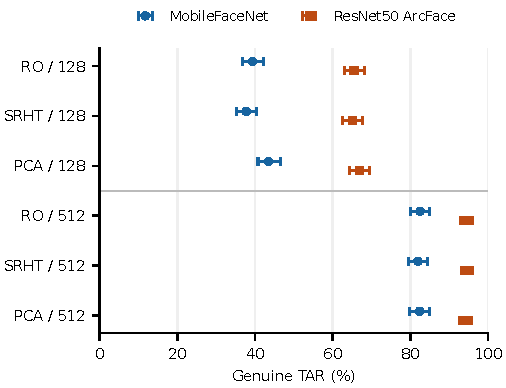
\includegraphics[width=\columnwidth]{cfp_recognition_ci.pdf}
\caption{Protected genuine recognition on screened CFP at the $10^{-3}$ validation-FAR target. Error bars are pointwise conditional 95\% identity-bootstrap intervals.}
\label{fig:cfp-recognition}\fignote{Matched inputs and protocols use encoder-specific fits and thresholds; PCA denotes PCA-guided RO, and row suffixes give bit lengths.}
\end{figure}
\begin{figure}[!tb]
\centering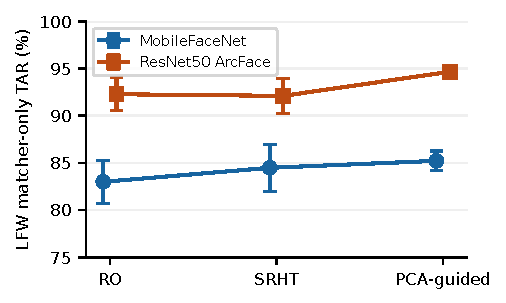
\includegraphics[width=\columnwidth]{lfw_recognition_sd.pdf}
\caption{LFW matcher-only recognition at 128 bits under official folds. Error bars show one standard deviation across five keys, not confidence intervals.}
\label{fig:lfw-recognition}\fignote{This extension evaluates recognition; it does not provide a second-encoder LFW attack result.}
\end{figure}
\begin{figure}[!tb]
\centering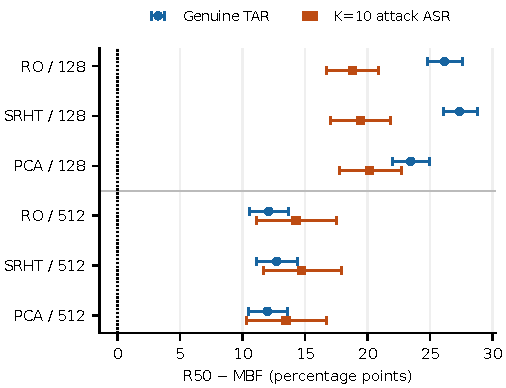
\includegraphics[width=\columnwidth]{paired_encoder_effects.pdf}
\caption{Paired ResNet50-minus-MobileFaceNet differences in genuine TAR and calibrated fresh-key ASR at $K=10$. Bars show pointwise conditional 95\% intervals; the dotted line marks zero.}
\label{fig:paired-encoder}\fignote{Positive differences mean higher acceptance, which has different implications for genuine and attack inputs.}
\end{figure}
\begin{figure}[!tb]
\centering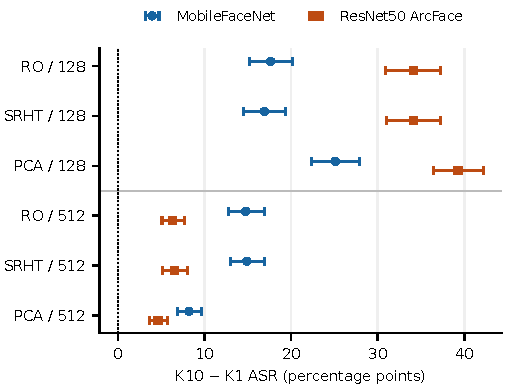
\includegraphics[width=\columnwidth]{paired_exposure_effects.pdf}
\caption{Paired $K=10$ minus $K=1$ calibrated fresh-key ASR differences for screened CFP. Bars show pointwise conditional 95\% intervals at the $10^{-3}$ validation-FAR target.}
\label{fig:paired-exposure}\fignote{Every plotted interval lies above zero; trials sharing an identity retain common bootstrap weights.}
\end{figure}
\begin{figure*}[!t]
\centering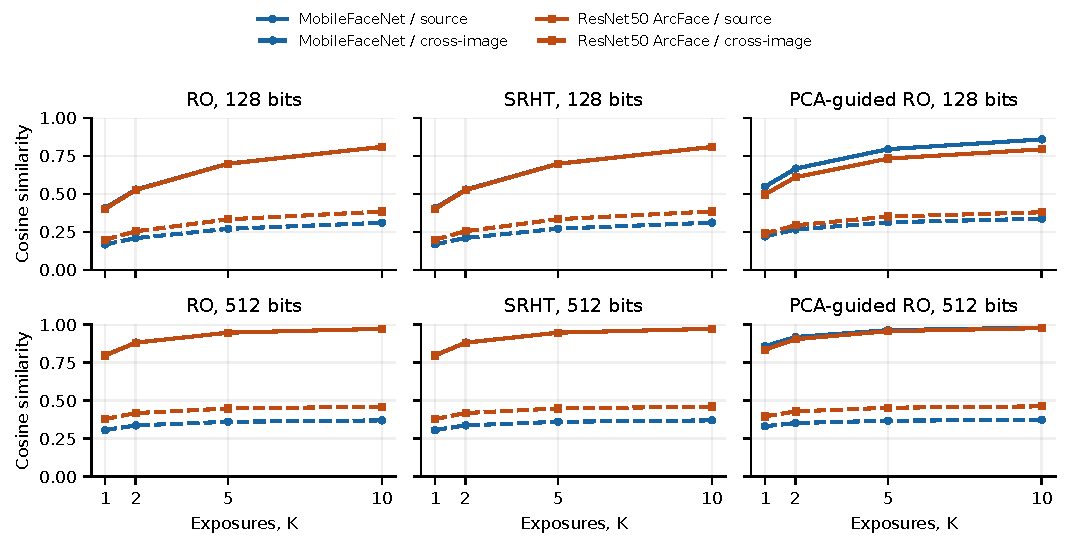
\includegraphics[width=.97\textwidth]{reconstruction_quality.pdf}
\caption{Calibrated reconstruction cosine over exposure count on screened CFP. Color identifies the encoder; solid and dashed lines distinguish the exposed source from the cross-image reference.}
\label{fig:reconstruction-quality}\fignote{Lines show point estimates, not uncertainty bands; cosine is unitless and is not attack acceptance.}
\end{figure*}
\begin{figure}[!tb]
\centering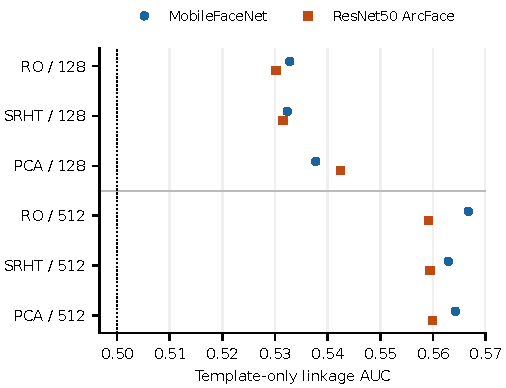
\includegraphics[width=\columnwidth]{linkage_comparison.pdf}
\caption{Template-only linkage at $K=10$ in the matched CFP replication. The dotted line denotes chance AUC; these descriptive means have no added confidence intervals.}
\label{fig:linkage-enc}\fignote{The learned score shows limited discrimination under this access model, which excludes old operators.}
\end{figure}

Figure~\ref{fig:linkage-enc} complements the inversion results with the template-only attacker. Figures~\ref{fig:enc-target128} and~\ref{fig:enc-target512} show how validation targets alter genuine acceptance, test FAR, and attack acceptance. At target $10^{-4}$, calibrated 512-bit $K=10$ ASR remains 69.59--70.54\% for MobileFaceNet and 89.01--90.09\% for ResNet50. These values belong to the matched replication, distinct from the original MobileFaceNet sweep. The stricter target reduces attack acceptance without demonstrating population FAR control at $10^{-4}$.
\begin{figure*}[!t]
\centering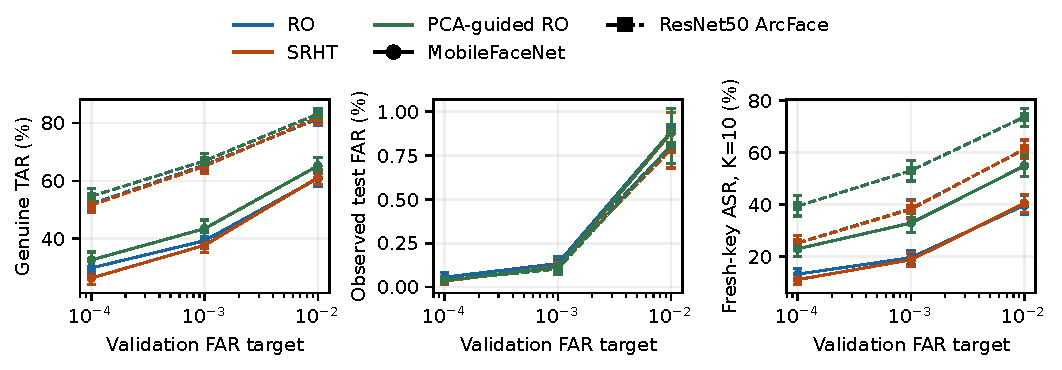
\includegraphics[width=\textwidth]{encoder_threshold_targets_128.pdf}
\caption{Matched CFP sensitivity at 128 bits: genuine TAR, observed test FAR, and calibrated $K=10$ fresh-key ASR at three validation-FAR targets. Error bars show pointwise conditional 95\% intervals.}
\label{fig:enc-target128}\fignote{Validation targets set the thresholds; the middle panel reports the separately observed test FAR.}
\end{figure*}
\begin{figure*}[!t]
\centering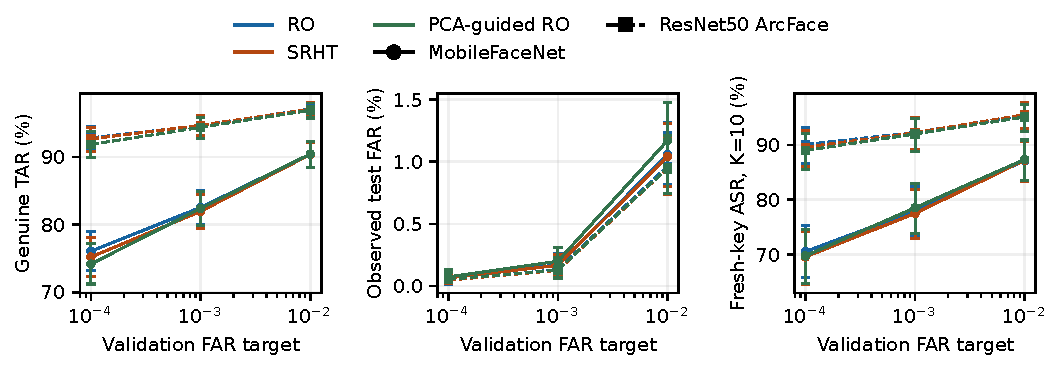
\includegraphics[width=\textwidth]{encoder_threshold_targets_512.pdf}
\caption{Matched CFP sensitivity at 512 bits with the same endpoints and validation-target convention as Fig.~\ref{fig:enc-target128}. Error bars show pointwise conditional 95\% intervals.}
\label{fig:enc-target512}\fignote{Substantial attack acceptance persists at the strictest evaluated validation target.}
\end{figure*}


\section{Discussion}\label{sec:discussion}


Rejecting an obsolete reference and resisting reconstruction are different outcomes in these experiments. The renewed matcher seldom accepts unchanged old bits, yet an estimate formed from historical templates and their operators can be accepted under an unexposed key. The paired contrasts between one and ten records show that repeated exposure supplies additional useful information within the evaluated protocols.

The relatively weak template-only linkage signal is consistent with the narrower information available to that attacker. Known-operator inversion exploits constraints that the linkage model cannot observe. A near-chance linkage score therefore offers little support for an irreversibility claim under operator compromise. Any security interpretation must specify both the exposed information and the interface through which an attack is submitted.


Every protected configuration in the matched CFP experiment achieves higher genuine acceptance with ResNet50. Fresh-key attack acceptance also increases at ten exposures, and all six paired encoder-difference intervals exclude zero on the positive side. The recognition gain does not resolve the reconstruction weakness observed for these projections. LFW provides additional evidence of improved recognition, but the available LFW attacks remain limited to MobileFaceNet.

These differences apply to the two evaluated checkpoints. Architecture, training data, and loss were not varied independently, and each encoder uses its own validation threshold. Moreover, the comparison does not hold genuine TAR exactly constant. The evidence therefore supports a conclusion about these pipelines, rather than a general association between recognition accuracy and insecurity.


The storage comparison gives a practical scale to the utility and security findings. For either encoder, storing a protected reference requires 16 or 64 bytes in place of a 2048-byte raw embedding. The equality of the two encoders' raw dimensions and protected lengths makes these payload savings directly comparable. They may matter for an edge device retaining many identities, although they say nothing by themselves about the rest of the system's memory requirement.

The 128-bit choice saves more storage but rejects more genuine comparisons. ResNet50 TAR on screened CFP rises from \RnetSmallTar{} at 128 bits to \RnetLargeTar{} at 512 bits; the longer representation also permits substantial reconstruction success. Selecting a length therefore requires an explicit judgment about genuine rejection and compromise risk, alongside payload. The storage result alone cannot establish either system efficiency or security.

End-to-end resource use includes image capture, detection, feature extraction, projection, matching, and key management. ResNet50 is included as a comparison encoder, not as a demonstrated substitute with the same device cost as MobileFaceNet. No measurement here establishes latency, peak memory, power, or energy on a kiosk or smart gadget.


Table~\ref{tab:priorcomparison} places the findings beside established protection and reconstruction studies. Pre-image and record-multiplicity attacks have prior examples~\cite{wang2021csa,li2014multiplicity}. The present empirical contribution connects exposure count to fresh-key acceptance, compares template lengths and encoders, and reports storage and genuine utility with the security outcomes. External methods were not rerun, so their reported success rates cannot support a direct ranking against these experiments.


Generalization remains limited by the use of two pretrained checkpoints and two celebrity datasets. Demographic variation, possible overlap with encoder-training data, and transfer to other capture conditions were not evaluated. Official recognition pairs and custom attack partitions also represent different populations and cannot be pooled. Differences between LFW and CFP may reflect preprocessing, selection, and calibration as well as pose.

The CFP screening procedure excluded 186 crops, and its post-hoc correspondence evidence and single-reviewer decisions constrain audit independence. Statistical coverage has further limits: the bootstrap holds fitted pipelines and thresholds fixed, omits refitting variability, and provides pointwise rather than multiplicity-adjusted intervals. The available impostor samples are too small to substantiate very-low-FAR population claims. Renewal and linkage findings similarly remain specific to the tested key schedules and classifiers.

The reconstructed input is a digital embedding. A camera attack would require additional image-generation and presentation tests. The accompanying source package contains protocol descriptions, numerical evidence, figure scripts, and checksums. The separate LFW replay archive contains frozen embeddings, operators, fitted PCA models, pair decisions, and validation checks. Full reproduction from photographs also requires the recorded datasets, model weights, and preprocessing environment.

\section{Conclusion and Future Work}\label{sec:conclusion}
Historical template compromise can remain consequential after a reference is renewed. In the evaluated pipelines, known old operators and repeated templates support reconstruction that passes a fresh-key matcher, despite rejection of unchanged old records and concealment of the fresh operator. At ten exposures, calibrated cross-image ASR in the matched CFP comparison is \MbfSmallAsr{} for MobileFaceNet and \RnetSmallAsr{} for ResNet50 at 128 bits; at 512 bits, the ranges are \MbfLargeAsr{} and \RnetLargeAsr{}. The separate original LFW MobileFaceNet study reaches \LfwBaselineAsr{} at 128 bits.

The same experiments place these security findings alongside recognition and storage. Both encoders support 16-byte and 64-byte references in place of 2048-byte raw embeddings. Although ResNet50 improves recognition, its higher utility does not confer reconstruction resistance under the tested exposure model. Compact-reference selection must therefore consider recognition, payload, and compromise jointly.

Further evaluation should measure latency, peak memory, energy, and operator storage for the complete pipeline on representative edge hardware. Additional encoders, larger impostor samples, independent correspondence review, and repeated model fitting would help assess the stability of the findings. Comparisons with alternative protection mechanisms should align genuine utility and attacker access. Image-generation and camera-level experiments would then be needed to assess attack interfaces beyond the digital embedding input studied here.
\FloatBarrier
\bibliographystyle{IEEEtran}
\bibliography{references}
\end{document}
